\documentclass[tikz, border={5pt, 15pt}]{standalone}

\begin{document}

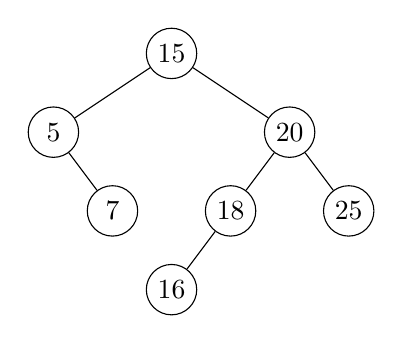
\begin{tikzpicture}[
	every node/.style={
		circle, draw,
		inner sep=0pt,
		text width=6mm,
		align=center
	},
	level distance=10mm,
	level 1/.style={sibling distance=30mm},
	level 2/.style={sibling distance=15mm}
]
\node{$15$}
child { node{$5$}
	child[missing]
	child { node{$7$} }
}
child { node{$20$}
	child { node{$18$}
		child { node{$16$} }
		child[missing]
	}
	child { node{$25$} }
};
\end{tikzpicture}

\end{document}
